%%%%%%%%%%%%%%%%%%%%%%%%%%%%%%%%%%
\section{引言}

本章演示如何插入图片并且创建标签进行交叉引用。

\section{tikz}

下图是使用tikz进行绘图的示例。

\begin{figure}[h]
    \centering
    \include*{images/neural}
    \caption{神经网络}
    \label{fig:basic_neural}
\end{figure}

\section{其他图像}

插入pdf图像。

\begin{figure}[htb]
    \centering
    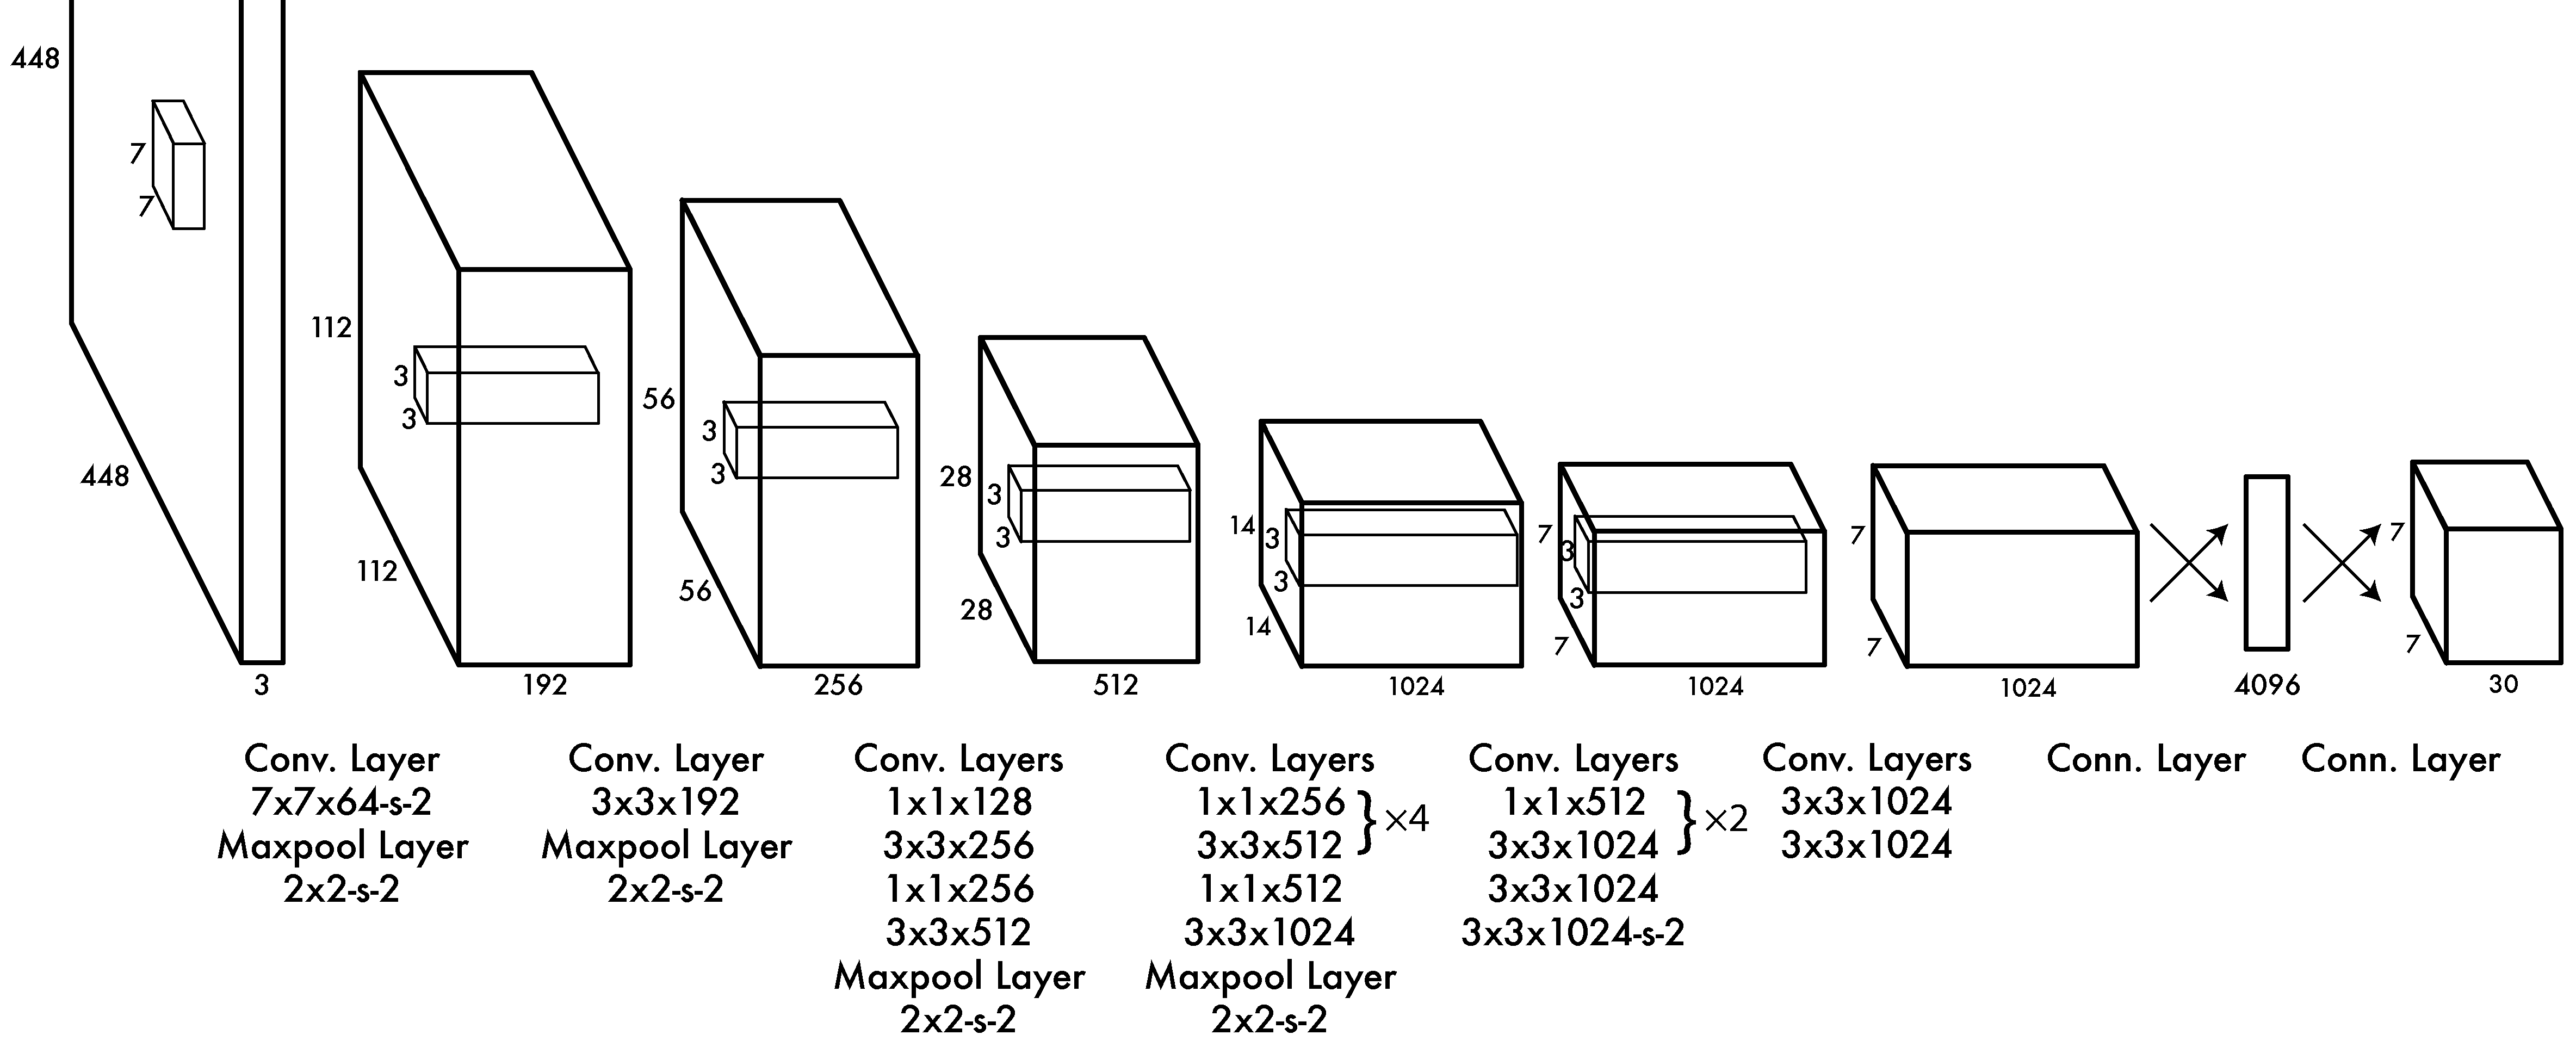
\includegraphics[width=0.8\linewidth]{images/yolo.pdf}
    \caption{YOLO网络结构图\cite{yolo}}
    \label{fig:yolo_struct}
\end{figure}

\section{tikz多图排版}

图\ref{fig:acti_func}由于太大有可能单独排版到一页。

\begin{figure}[htbp]
    \centering
    \pgfplotsset{width={\linewidth}}
    \begin{minipage}{0.32\linewidth}
        \centering
        \include*{images/sigmoid}
    \end{minipage}
    \begin{minipage}{0.32\linewidth}
        \centering
        \include*{images/relu}
    \end{minipage}
    \begin{minipage}{0.32\linewidth}
        \centering
        \include*{images/silu}
    \end{minipage}
    
    \begin{minipage}{0.32\linewidth}
        \centering
        \include*{images/tanh}
    \end{minipage}
    \begin{minipage}{0.32\linewidth}
        \centering
        \include*{images/leaky_relu}
    \end{minipage}
    \begin{minipage}{0.32\linewidth}
        \centering
        \include*{images/mish}
    \end{minipage}

    \begin{minipage}{0.32\linewidth}
        \centering
        \include*{images/d-sigmoid}
    \end{minipage}
    \begin{minipage}{0.32\linewidth}
        \centering
        \include*{images/d-relu}
    \end{minipage}
    \begin{minipage}{0.32\linewidth}
        \centering
        \include*{images/d-silu}
    \end{minipage}
    
    \begin{minipage}{0.32\linewidth}
        \centering
        \include*{images/d-tanh}
    \end{minipage}
    \begin{minipage}{0.32\linewidth}
        \centering
        \include*{images/d-leaky_relu}
    \end{minipage}
    \begin{minipage}{0.32\linewidth}
        \centering
        \include*{images/d-mish}
    \end{minipage}

    \caption{常见的激活函数及其导函数图像}
    \label{fig:acti_func}
\end{figure}

